% questions.tex —— 2005 年·全国卷Ⅰ·文科 · 题目内容片段（无答案）
% 由 tools/generate_projects.py 依来源总账自 2005/2005_数学真题_全国1文_试题.md 生成，勿手改（改源 MD 后重跑）


\gkpart{数学}

\begin{gktip}
\textbf{来源说明}：本题面依据固定源 PDF 两页 A3 题面逐题转录，原卷印刷页码 248–249。固定源不附答案，答案和解析均由本库独立复算。

\textbf{图形说明}：第 4、18 题的原卷图形关系重绘为 TikZ/PGFPlots 矢量图。图形标记所指的 PNG 不随仓库保存。
\end{gktip}

\gkpart{一、选择题}

\begin{question}
\gkti{1}设 $I$ 为全集，$S_1\text{、}S_2\text{、}S_3$ 是 $I$ 的三个非空子集且 $S_1\cup S_2\cup S_3=I$，则下面论断正确的是\mbox{（　　）}

（A）$\complement_I S_1\cap(S_2\cup S_3)=\varnothing$\quad（B）$S_1\subseteq(\complement_I S_2\cap\complement_I S_3)$

（C）$\complement_I S_1\cap\complement_I S_2\cap\complement_I S_3=\varnothing$\quad（D）$S_1\subseteq(\complement_I S_2\cup\complement_I S_3)$

\end{question}
\begin{question}
\gkti{2}一个与球心距离为 $1$ 的平面截球所得的圆面面积为 $\pi$，则球的表面积为\mbox{（　　）}

（A）$8\sqrt2\pi$\quad（B）$8\pi$\quad（C）$4\sqrt2\pi$\quad（D）$4\pi$

\end{question}
\begin{question}
\gkti{3}函数 $f(x)=x^3+ax^2+3x-9$，已知 $f(x)$ 在 $x=-3$ 时取得极值，则 $a=$\mbox{（　　）}

（A）$2$\quad（B）$3$\quad（C）$4$\quad（D）$5$

\Needspace{0.4\textheight}
\end{question}
\begin{question}
\gkti{4}如图，在多面体 $ABCDEF$ 中，已知 $ABCD$ 是边长为 $1$ 的正方形，且 $\triangle ADE\text{、}\triangle BCF$ 均为正三角形，$EF\parallel AB$，$EF=2$，则该多面体的体积为\mbox{（　　）}
\nopagebreak[4]
\begin{center}% 2005 年全国卷Ⅰ文科第 4 题：多面体 ABCDEF
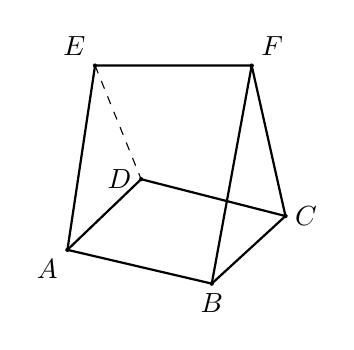
\begin{tikzpicture}[>=stealth,scale=0.78]
  \coordinate (A) at (0,0); \coordinate (B) at (2.35,-0.55);
  \coordinate (C) at (3.55,0.55); \coordinate (D) at (1.2,1.15);
  \coordinate (E) at (0.45,3.0); \coordinate (F) at (3.0,3.0);
  \draw[thick] (A)--(B)--(C)--(D)--cycle;
  \draw[thick] (A)--(E)--(F)--(B);
  \draw[thick] (C)--(F);
  \draw[dashed] (E)--(D) (D)--(C);
  \fill (A) circle (1pt) node[below left] {$A$};
  \fill (B) circle (1pt) node[below] {$B$};
  \fill (C) circle (1pt) node[right] {$C$};
  \fill (D) circle (1pt) node[left] {$D$};
  \fill (E) circle (1pt) node[above left] {$E$};
  \fill (F) circle (1pt) node[above right] {$F$};
\end{tikzpicture}
\end{center}
\nopagebreak[4]
（A）$\dfrac{\sqrt2}{3}$\quad（B）$\dfrac{\sqrt3}{3}$\quad（C）$\dfrac43$\quad（D）$\dfrac32$

\end{question}
\begin{question}
\gkti{5}已知双曲线 $\dfrac{x^2}{a^2}-y^2=1\ (a>0)$ 的一条准线与抛物线 $y^2=-6x$ 的准线重合，则该双曲线的离心率为\mbox{（　　）}

（A）$\dfrac{\sqrt3}{2}$\quad（B）$\dfrac32$\quad（C）$\dfrac{\sqrt6}{2}$\quad（D）$\dfrac{2\sqrt3}{3}$

\end{question}
\begin{question}
\gkti{6}当 $0<x<\dfrac{\pi}{2}$ 时，函数

\nopagebreak[4]
\[
f(x)=\frac{1+\cos2x+8\sin^2x}{\sin2x}
\]

的最小值为\mbox{（　　）}

（A）$2$\quad（B）$2\sqrt3$\quad（C）$4$\quad（D）$4\sqrt3$

\end{question}
\begin{question}
\gkti{7}$y=\sqrt{2x-x^2}\ (1\leqslant x\leqslant2)$ 的反函数是\mbox{（　　）}

（A）$y=1+\sqrt{1-x^2}\ (-1\leqslant x\leqslant1)$\quad（B）$y=1+\sqrt{1-x^2}\ (0\leqslant x\leqslant1)$

（C）$y=1-\sqrt{1-x^2}\ (-1\leqslant x\leqslant1)$\quad（D）$y=1-\sqrt{1-x^2}\ (0\leqslant x\leqslant1)$

\end{question}
\begin{question}
\gkti{8}设 $0<a<1$，函数 $f(x)=\log_a(a^{2x}-2a^x-2)$，则使 $f(x)<0$ 的 $x$ 取值范围是\mbox{（　　）}

（A）$\mathbb R$\quad（B）$(0,+\infty)$\quad（C）$(-\infty,\log_a3)$\quad（D）$(\log_a3,+\infty)$

\end{question}
\begin{question}
\gkti{9}在坐标平面上，不等式组

\nopagebreak[4]
\[
\begin{cases}
y\geqslant x-1,\\
y\leqslant-3|x|+1
\end{cases}
\]

所表示的平面区域的面积为\mbox{（　　）}

（A）$\sqrt2$\quad（B）$\dfrac32$\quad（C）$\dfrac{3\sqrt2}{2}$\quad（D）$2$

\end{question}
\begin{question}
\gkti{10}在 $\triangle ABC$ 中，已知 $\tan\dfrac{A+B}{2}=\sin C$，给出以下四个论断：① $\tan A\cdot\cot B=1$；② $0<\sin A+\sin B\leqslant2$；③ $\sin^2A+\cos^2B=1$；④ $\cos^2A+\cos^2B=\sin^2C$。其中正确的是\mbox{（　　）}

（A）①③\quad（B）②④\quad（C）①④\quad（D）②③

\end{question}
\begin{question}
\gkti{11}点 $O$ 是三角形 $ABC$ 所在平面内的一点，满足 $\overrightarrow{OA}\cdot\overrightarrow{OB}=\overrightarrow{OB}\cdot\overrightarrow{OC}=\overrightarrow{OC}\cdot\overrightarrow{OA}$，则点 $O$ 是 $\triangle ABC$ 的\mbox{（　　）}

（A）三个内角的角平分线的交点\quad（B）三条边的垂直平分线的交点

（C）三条中线的交点\quad（D）三条高的交点

\end{question}
\begin{question}
\gkti{12}设直线 $l$ 过点 $(-2,0)$，且与圆 $x^2+y^2=1$ 相切，则 $l$ 的斜率是\mbox{（　　）}

（A）$\pm1$\quad（B）$\pm\dfrac12$\quad（C）$\pm\dfrac{\sqrt3}{3}$\quad（D）$\pm\sqrt3$

\end{question}
\gkpart{二、填空题}

\begin{question}
\gkti{13}若正整数 $m$ 满足 $10^{m-1}<2^{512}<10^m$，则 $m=$\gkblank{}。（$\lg2\approx0.3010$）

\end{question}
\begin{question}
\gkti{14}$\left(x-\dfrac1x\right)^8$ 的展开式中，常数项为\gkblank{}。（用数字作答）

\end{question}
\begin{question}
\gkti{15}从 $6$ 名男生和 $4$ 名女生中，选出 $3$ 名代表，要求至少包含 $1$ 名女生，则不同的选法有\gkblank{}种。

\end{question}
\begin{question}
\gkti{16}在正方体 $ABCD-A'B'C'D'$ 中，过对角线 $BD'$ 的一个平面交 $AA'$ 于 $E$，交 $CC'$ 于 $F$，则：

① 四边形 $BFD'E$ 一定是平行四边形；

② 四边形 $BFD'E$ 有可能是正方形；

③ 四边形 $BFD'E$ 在底面 $ABCD$ 内的投影一定是正方形；

④ 平面 $BFD'E$ 有可能垂直于平面 $BB'D$。

以上结论正确的为\gkblank{}。（写出所有正确结论的编号）

\end{question}
\gkpart{三、解答题}

\begin{question}
\gkti{17}设函数 $f(x)=\sin(2x+\varphi)\ (-\pi<\varphi<0)$，$y=f(x)$ 图象的一条对称轴是直线 $x=\dfrac{\pi}{8}$。

（1） 求 $\varphi$；

（2） 求函数 $y=f(x)$ 的单调增区间；

（3） 画出函数 $y=f(x)$ 在区间 $[0,\pi]$ 上的图象。

\Needspace{0.4\textheight}
\end{question}
\begin{question}
\gkti{18}已知四棱锥 $P-ABCD$ 的底面为直角梯形，$AB\parallel DC$，$\angle DAB=90^\circ$，$PA\perp$ 底面 $ABCD$，且 $PA=AD=DC=\dfrac12AB=1$，$M$ 是 $PB$ 的中点。
\nopagebreak[4]
\begin{center}% 2005 年全国卷Ⅰ文科第 18 题：直角梯形底面的四棱锥
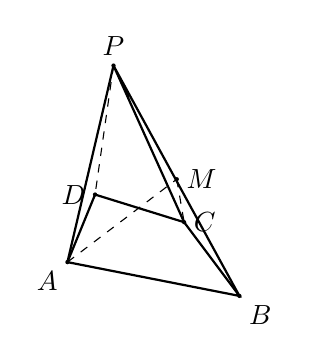
\begin{tikzpicture}[>=stealth,scale=0.78]
  \coordinate (A) at (0,0); \coordinate (B) at (2.8,-0.55);
  \coordinate (C) at (1.9,0.65); \coordinate (D) at (0.45,1.1);
  \coordinate (P) at (0.75,3.2); \coordinate (M) at (1.78,1.35);
  \draw[thick] (A)--(B)--(C)--(D)--cycle;
  \draw[thick] (P)--(A) (P)--(B) (P)--(C);
  \draw[dashed] (P)--(D) (A)--(M) (M)--(C);
  \fill (P) circle (1pt) node[above] {$P$};
  \fill (A) circle (1pt) node[below left] {$A$};
  \fill (B) circle (1pt) node[below right] {$B$};
  \fill (C) circle (1pt) node[right] {$C$};
  \fill (D) circle (1pt) node[left] {$D$};
  \fill (M) circle (1pt) node[right] {$M$};
\end{tikzpicture}
\end{center}
\nopagebreak[4]
（1） 证明：面 $PAD\perp$ 面 $PCD$；

（2） 求 $AC$ 与 $PB$ 所成的角；

（3） 求面 $AMC$ 与面 $BMC$ 所成二面角的大小。

\end{question}
\begin{question}
\gkti{19}设正项等比数列 $\{a_n\}$ 的首项 $a_1=\dfrac12$，前 $n$ 项和为 $S_n$，且

\nopagebreak[4]
\[
2^{10}S_{30}-(2^{10}+1)S_{20}+S_{10}=0\text{。}
\]

（1） 求 $\{a_n\}$ 的通项；

（2） 求 $\{nS_n\}$ 的前 $n$ 项和 $T_n$。

\end{question}
\begin{question}
\gkti{20}$9$ 粒种子分种在甲、乙、丙 $3$ 个坑内，每坑 $3$ 粒，每粒种子发芽的概率为 $0.5$。若一个坑内至少有 $1$ 粒种子发芽，则这个坑不需要补种；若一个坑里的种子都没发芽，则这个坑需要补种，求：

（1） 甲坑不需要补种的概率；

（2） $3$ 个坑中恰有 $1$ 个坑不需要补种的概率；

（3） 有坑需要补种的概率。（精确到 $0.001$）

\end{question}
\begin{question}
\gkti{21}已知椭圆的中心为坐标原点 $O$，焦点在 $x$ 轴上，斜率为 $1$ 且过椭圆右焦点 $F$ 的直线交椭圆于 $A\text{、}B$ 两点，$\overrightarrow{OA}+\overrightarrow{OB}$ 与 $\vec a=(3,-1)$ 共线。

（1） 求椭圆的离心率；

（2） 设 $M$ 为椭圆上任意一点，且 $\overrightarrow{OM}=\lambda\overrightarrow{OA}+\mu\overrightarrow{OB}\ (\lambda,\mu\in\mathbb R)$，证明 $\lambda^2+\mu^2$ 为定值。

\end{question}
\begin{question}
\gkti{22}设函数

\nopagebreak[4]
\[
f(x)=x\log_2x+(1-x)\log_2(1-x)\qquad(0<x<1)\text{，}
\]

（1） 求 $f(x)$ 的最小值；

\Needspace{5\baselineskip}
（2） 设正数 $p_1,p_2,p_3,\ldots,p_{2n}$ 满足 $p_1+p_2+p_3+\cdots+p_{2n}=1$，证明

\nopagebreak[4]
\[
p_1\log_2p_1+p_2\log_2p_2+\cdots+p_{2n}\log_2p_{2n}\geqslant-n\text{。}
\]

\end{question}